\documentclass[a4paper]{report}
\usepackage[utf8]{inputenc}
\usepackage[portuguese]{babel}
\usepackage{hyperref}
\usepackage{a4wide}
\hypersetup{pdftitle={PCP - OpenMP e OpenMPI},
pdfauthor={João Teixeira, José Ferreira},
colorlinks=true,
urlcolor=blue,
linkcolor=black}
\usepackage{subcaption}
\usepackage{listings}
\usepackage{booktabs}
\usepackage{multirow}
\usepackage{appendix}
\usepackage{tikz}
\usepackage{authblk}
\usepackage{bashful}
\usepackage{verbatim}
\usepackage{amssymb}
\usepackage{multirow}
\usepackage{mwe}
\usepackage[parfill]{parskip}
\usetikzlibrary{positioning,automata,decorations.markings}
\AfterEndEnvironment{figure}{\noindent\ignorespaces}
\AfterEndEnvironment{table}{\noindent\ignorespaces}

\begin{document}

\title{Paradigmas de Computação Paralela\\Bucket Sort com OpenMP e OpenMPI}
\author{João Teixeira (A85504) \and José Filipe Ferreira (A83683)}
\date{\today}

\begin{center}
    \begin{minipage}{0.75\linewidth}
        \centering
        
\includegraphics[width=0.4\textwidth]{images/eng.jpeg}\par\vspace{1cm}
        \vspace{1.5cm}
        \href{https://www.uminho.pt/PT}
        {\color{black}{\scshape\LARGE Universidade do Minho}} \par
        \vspace{1cm}
        \href{https://www.di.uminho.pt/}
        {\color{black}{\scshape\Large Departamento de Informática}} \par
        \vspace{1.5cm}
        \maketitle
    \end{minipage}
\end{center}

\tableofcontents

\pagebreak

\chapter{Introdução}
O algoritmo escolhido para o projeto da unidade curricular de Computação
Paralela e Distribuída foi o \textit{Bucket Sort}.

Numa primeira fase do trabalho desenvolvemos uma versão sequencial do projeto e
procedemos ao \textit{benchmarking} do programa resultante. Em seguida
convertemos a implementação sequencial numa versão com utilização de memoria
partilhada fazendo uso de \textit{OpenMP} e comparamos o resultado com a versão
sequencial desenvolvida anteriormente.

Nesta segunda fase desenvolvemos uma nova versao do \textit{bucket sort} fazendo
uso de memoria distribuída com o \textit{OpenMPI} comparando os resultados do
benchmarking deste algoritmo com os resultados obtidos na fase anterior.

De notar que todos os benchmarks descritos foram efeutados em nós do tipo 642 do
cluster \textit{SeARCH}, e todos os executáveis foram compilados o
\textit{MPIcc} na versão 1.8.1 do \textit{OpenMPI}, utilizando a versão
7.2.0 do \textit{gcc}, e com as flags \textit{-O3 -std=c11} para garantir
a maior consistência entre os diferentes benchmarks. Na
ausência de indicação, os benchmarks foram efetuados com um input de 100000000
de elementos aleatórios, entre -1000 e 500000.



\chapter{OpenMPI} \label{chap:ompi}

\section{Descrição da Implementação}
O algoritmo de Bucket Sort adaptado para \textit{MPI} divide-se em quatro fases,
divisão dos elementos em chunks para serem enviados para os diferentes
processos, separação dos elementos pelos diversos baldes, junção e ordenação dos
baldes dos diferentes processos, e por fim a agregação dos baldes ordenados num
array final. A segunda e terceira fase é feita em paralelo, enquanto que a
primeira e ultima são realizadas apenas por um processo.

Numa implementação inicial do algoritmo paralelo, apenas paralelizamos a
segunda fase, onde os resultados e implementação são explicados em mais detalhe
no apêndice \ref{apx:slowpar}.

A nossa implementação realiza a primeira fase de divisão dos elementos em chunks
num único processo, onde é difundido o máximo e o mínimo dos elementos a
ordenar, e o tamanho dos buffers que os diferentes processos devem ter para
garantir a boa recessão do chunk que lhe corresponde. Depois desta difusão, é
enviado a todos os processos o chunk correspondendo, realizando P envios, um por
cada processo, com o tamanho máximo de (P/N + 1) * 4 bytes, onde P é o número de
processos e o N corresponde ao número de elementos total a ordenar.

Recebido pelos processos os chunks respetivos, cada um vai percorrer os
elementos recebidos, atribuindo-o cada um ao respetivo balde. Depois de todos os
baldes preenchidos, cada processo vai enviar cada balde para um processo que
irá juntar ao mesmo balde vindo dos outros processos. Esta distribuição é
efetuada para que todos os processos recebam um número equilibrado de
buckets, onde cada processo irá receber B/P baldes, caso existam mais baldes
que processos, senão irá receber ou um ou zero baldes, dependendo do seu id.
Aqui cada processo irá realizar B envios, com um máximo (P/N + 1) * 4 bytes,
com B sendo o número de baldes, e o P e N indicados acima.

Finda a recessão de todos os buckets que um processo tem para processar, estes
irão proceder à ordenação destes, e finda esta são agrupados num só array os
baldes consecutivos e ordenados. Depois deste passo, é enviado este array para o
processo que tinha inicialmente feito a distribuição dos chunks. É realizado um
envio no máximo com N * 4 bytes.

Neste processo que recebeu os arrays de todos os processos que trataram de algum
bucket, são agrupados e retornado o resultado final.

\begin{figure}[h]
    \centering
    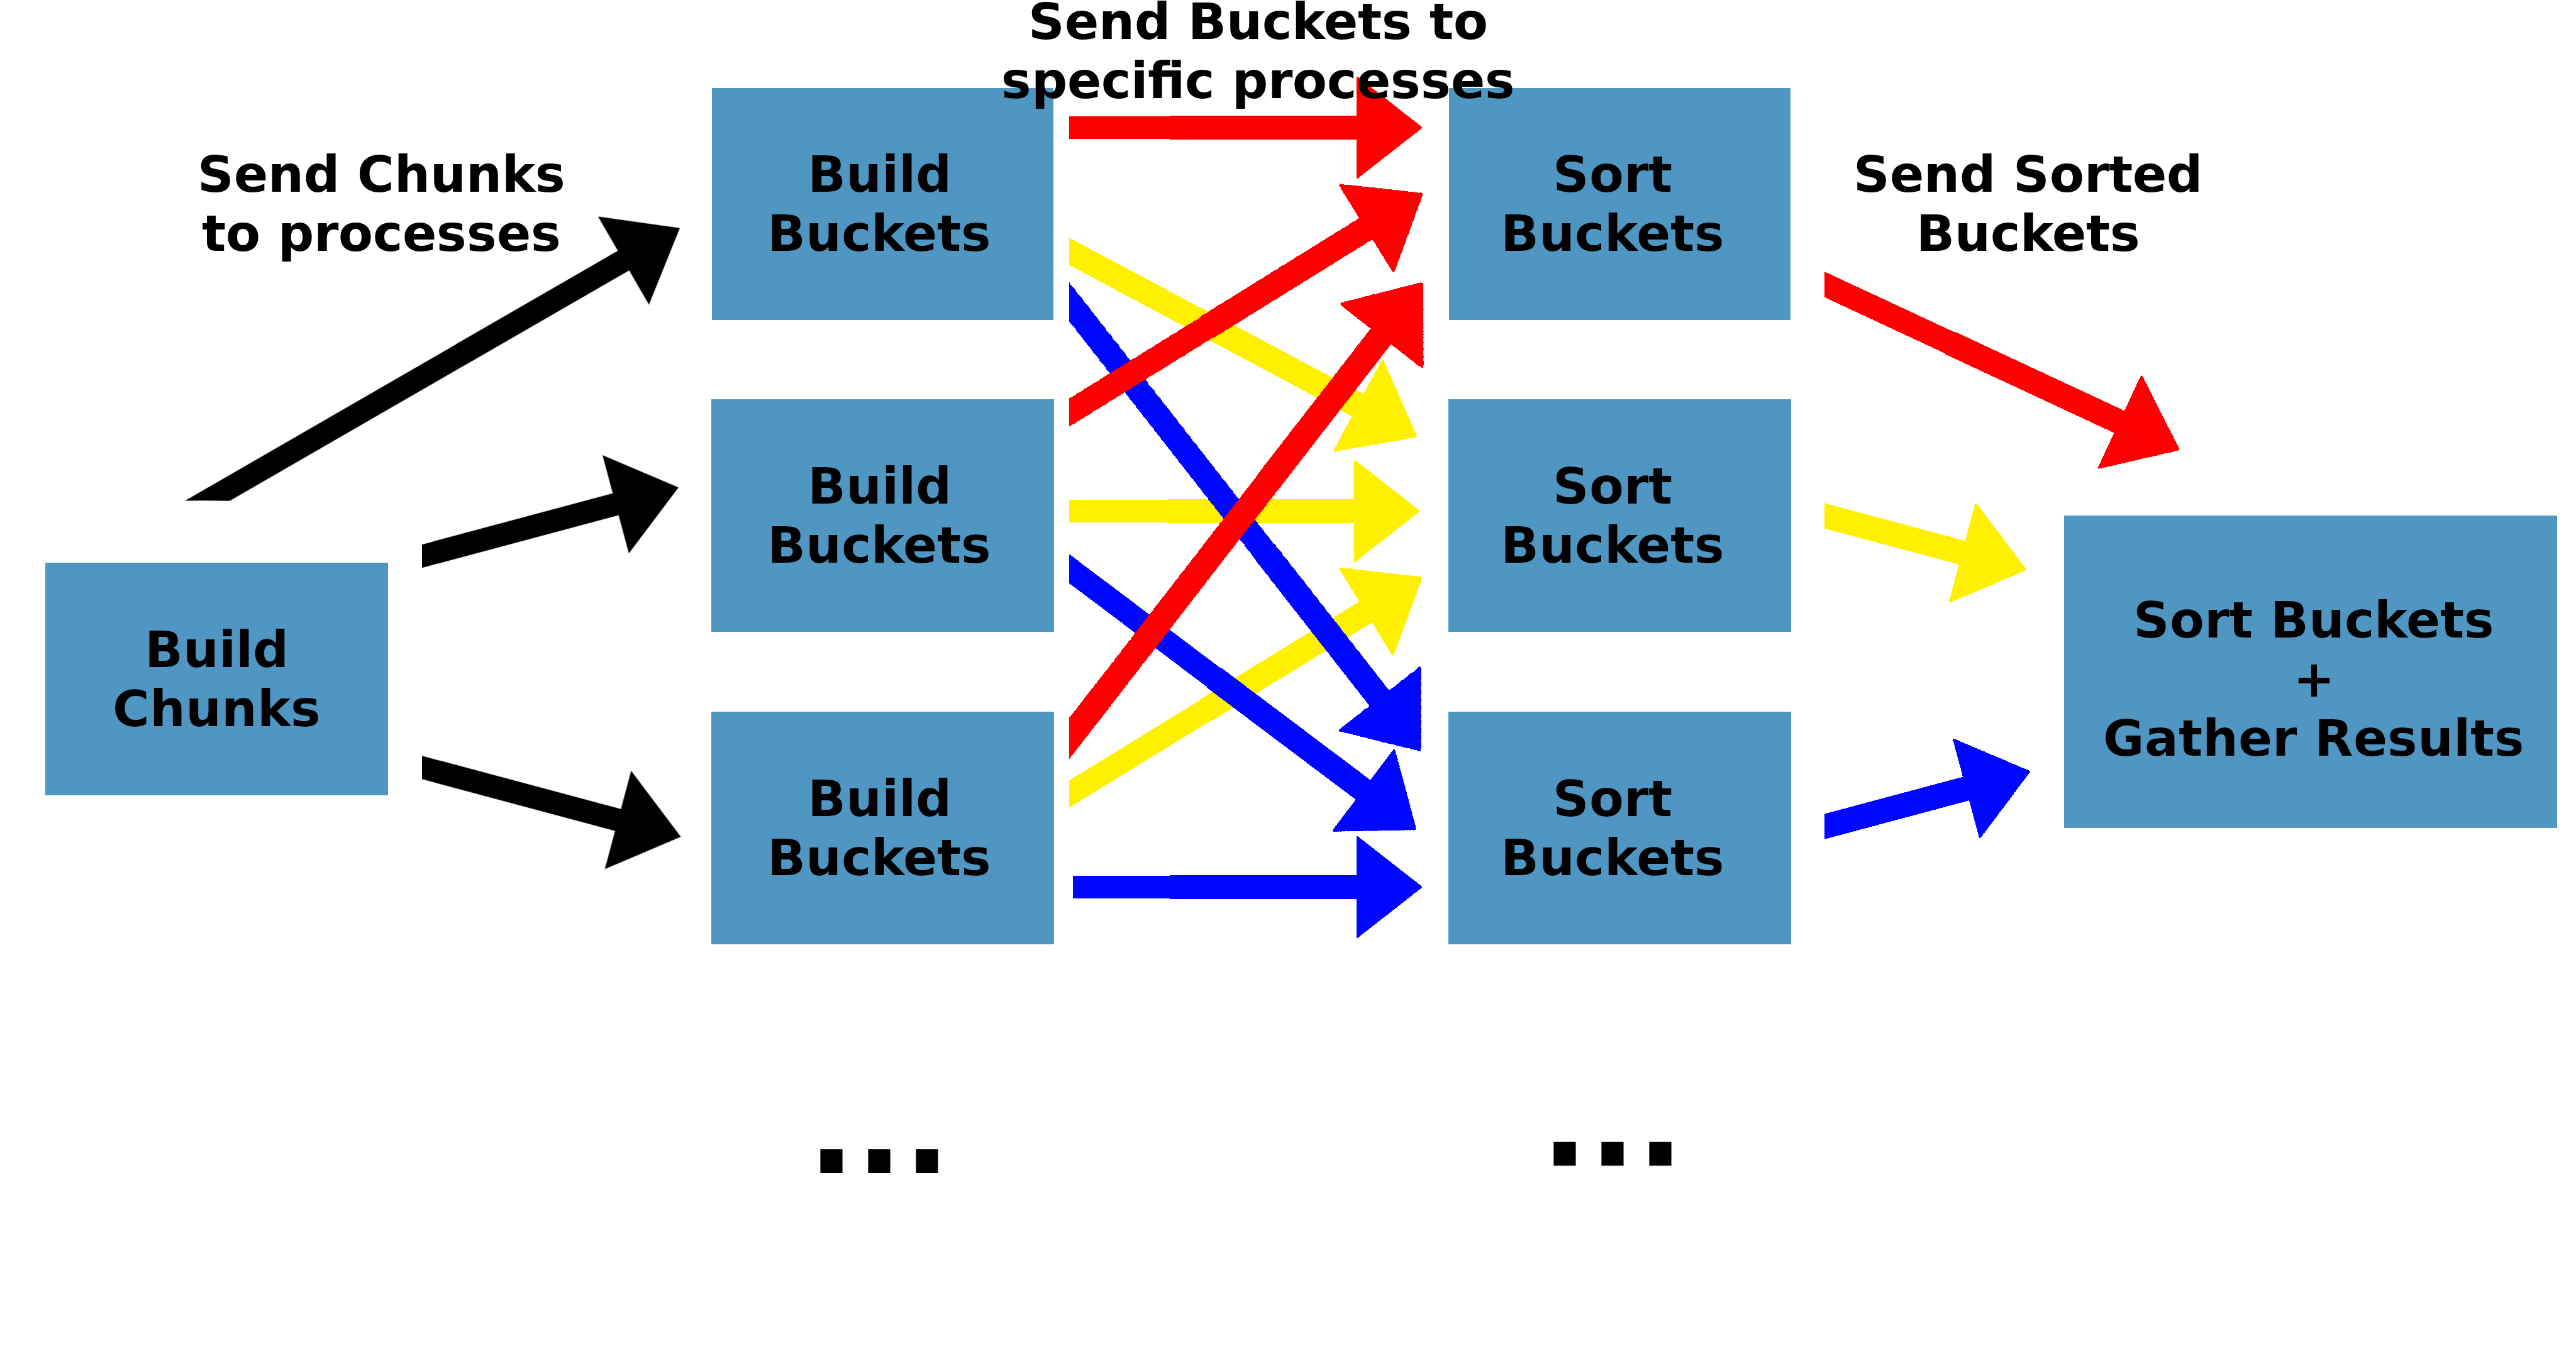
\includegraphics[width=0.6\textwidth]{images/esquemas/algoritmo_graph2.png}
    \caption{Arquitetura da Solução}
\end{figure}

\pagebreak
\section{Análise dos resultados}
\begin{table}[h]
    \centering
    \begin{tabular}{|c|c|}
        \hline
        Processes & Time(Seconds) \\ \hline
        2         & 10,170775     \\ \hline
        4         & 10,061176     \\ \hline
        8         & 6,581753      \\ \hline
        16        & 2,5495        \\ \hline
        32        & 6,165742      \\ \hline
    \end{tabular}
    \caption{\label{tab:Times}Tempos de execução do algoritmo, com 10 baldes}
\end{table}
\begin{figure}[h]
    \centering
    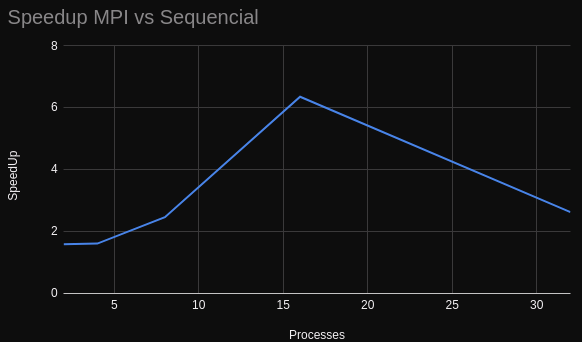
\includegraphics[width=0.6\textwidth]{images/speedupseq.jpeg}
    \caption{Speedup MPI vs Sequencial}
    \label{img:smpi}
\end{figure}

Como visto na tabela \ref{tab:Times} passar de dois para quatro não
se viram grandes ganhos, pois a carga computacional por processo ainda
é alta, e são realizadas 2 vezes mais comunicações entre processos,
de tamanho ainda considerável. Para 8 e 16 processos vemos speedups
mais substanciais, com a carga computacional do algoritmo a ser
mais distribuida, e a as comunicações entre processos a ser cada
vez mais rápida, graças à diminuição do comprimento das mensagens transmitidas.

Para os 32 processos, vemos um aumento dos tempos de execução, pois como quando
o número de processos é maior que o número de processos, muitos deles têm uma
carga computacional muito baixa e tendo uma carga muito pouco balanceada entre
processos, fazendo notar-se mais o overhead de ter processos extra.

A versão sequencial utilizada para o calculo dos speedups na figura
\ref{img:smpi} foi a versão mais
rápida da fase anterior, com um tempo de execução para o mesmo input de
16.209999 segundos. 
\section{Variação do número de baldes}

Com a análise dos resultados da execução do programa com 10 baldes, vemos que
para um número de processos maior que o número de baldes existe uma grande
penalização. Para tentar um melhor balanceamento de carga, efetuamos testes com
diferentes número de baldes, em relação ao número de processos.

\begin{table}[h]
    \centering
    \begin{tabular}{|l|l|l|l|l|}
        \hline
   & 1/2x      & 1x       & 2x        & 4x       \\ \hline
        2  & -         & 8,901732 & 14,998655 & 8,239823 \\ \hline
        4  & 10,124461 & 9,067322 & 9,492485  & 7,405527 \\ \hline
        8  & 4,936002  & 4,676249 & 7,602705  & 7,210904 \\ \hline
        16 & 2,908431  & 3,643568 & 4,996264  & 4,844009 \\ \hline
        32 & 4,103812  & 2,907007 & 3,711787  & 6,2266   \\ \hline
    \end{tabular}
    \caption{\label{tab:varb}Tempos de execução do algoritmo, com o número de
    baldes como um múltiplo de número de processos}
\end{table}

Como podemos ver, quando o número de baldes é metade do número de processos, a
carga ainda não é balanceada e embora sejam tempos mais baixos que nas execuções
de 10 baldes fixos, não representam o melhor caso. Com a carga melhor
distribuída, onde cada processo irá processar um balde apenas, vemos as melhores
execuções. Acima disto, o overhead das comunicações acrescidas pelo aumento do
número de baldes não compensa o esforço extra.

\appendix

\chapter{Algoritmo em dois nodos distintos}

Fazendo uso da flag do \textit{mpirun} \textit{--map-by node}, que aloca de
forma equilibrada os processos pelos nodos existentes a correr, fizemos alguns
testes para ver como se comportava o algoritmo quando existe o custo extra da
comunicação entre nodos. Como visto na tabela \ref{tab:nodes}, e comparando com os tempos da
tabela \ref{tab:Times}, vemos que para este algoritmo e carga, a carga
computacional não é suficiente para dissolver o custo acrescido nas comunicações
entre máquinas.

\begin{table}[h]
    \centering
    \begin{tabular}{ccc}
        Processes & Time(Seconds) & Speedup      \\
        2         & 20,496617     & 0,4962172538 \\
        4         & 12,927193     & 0,7782954892 \\
        8         & -             & -            \\
        16        & 7,983936      & 0,3193287121 \\
        32        & 7,414105      & 0,8316232371
    \end{tabular}
    \caption{Tempos de execução do algoritmo em dois nodos}
    \label{tab:nodes}
\end{table}

\chapter{OpenMP vs OpenMPI}
\begin{table}[h]
    \centering
    \begin{tabular}{|c|c|c|c|}
        \hline
        Workers & OpenMP    & OpenMPI  & Speedup      \\ \hline
        2       & 11,403177 & 8,901732 & 1,28100655   \\ \hline
        4       & 6,880816  & 9,067322 & 0,7588586796 \\ \hline
        8       & 4,622566  & 4,676249 & 0,9885200724 \\ \hline
        16      & 2,362948  & 3,643568 & 0,6485258406 \\ \hline
        32      & 2,363651  & 2,907007 & 0,8130874814 \\ \hline
    \end{tabular}
    \caption{Tempos de OpenMP vs OpenMPI}
    \label{tab:ompi}
\end{table}

Analisando em detalhe a tabela \ref{tab:ompi} podemos ver que para o mesmo
número de processos ou threads, conseguimos tempos semelhantes. Como a nossa
implementação do OpenMP replica trabalho, o que não nos permitiu ter speedups em
relação à versão sequencial, a não replicação do trabalho foi suficiente para
amortizar o overhead da comunicação entre processos da versão OpenMPI.

\chapter{Primeira Implementação do algoritmo} \label{apx:slowpar}

A primeira implementação do algoritmo em relação à versão final toma uma
abordagem mais conservadora sobre as comunicações, reduzindo-as, sacrificando a
quantidade de código paralelo a ser corrido. Aqui apenas é paralelizada a
segunda fase do algoritmo, as comunicações entre processos passam a ser apenas P
comunicações de máximo (N/P + 1) * 4 bytes para a distribuição de chunks pelos
processos, com P sendo o número de processos e N o número de elementos total a
ordenar. Depois dos chunks distribuidos, cada processo forma os seus baldes e os
envia ao processo que dividiu os chunks inicialmente e este irá proceder à fase
de ordenação e junção dos baldes ordenados para retornar.

\begin{figure}[h]
    \centering
    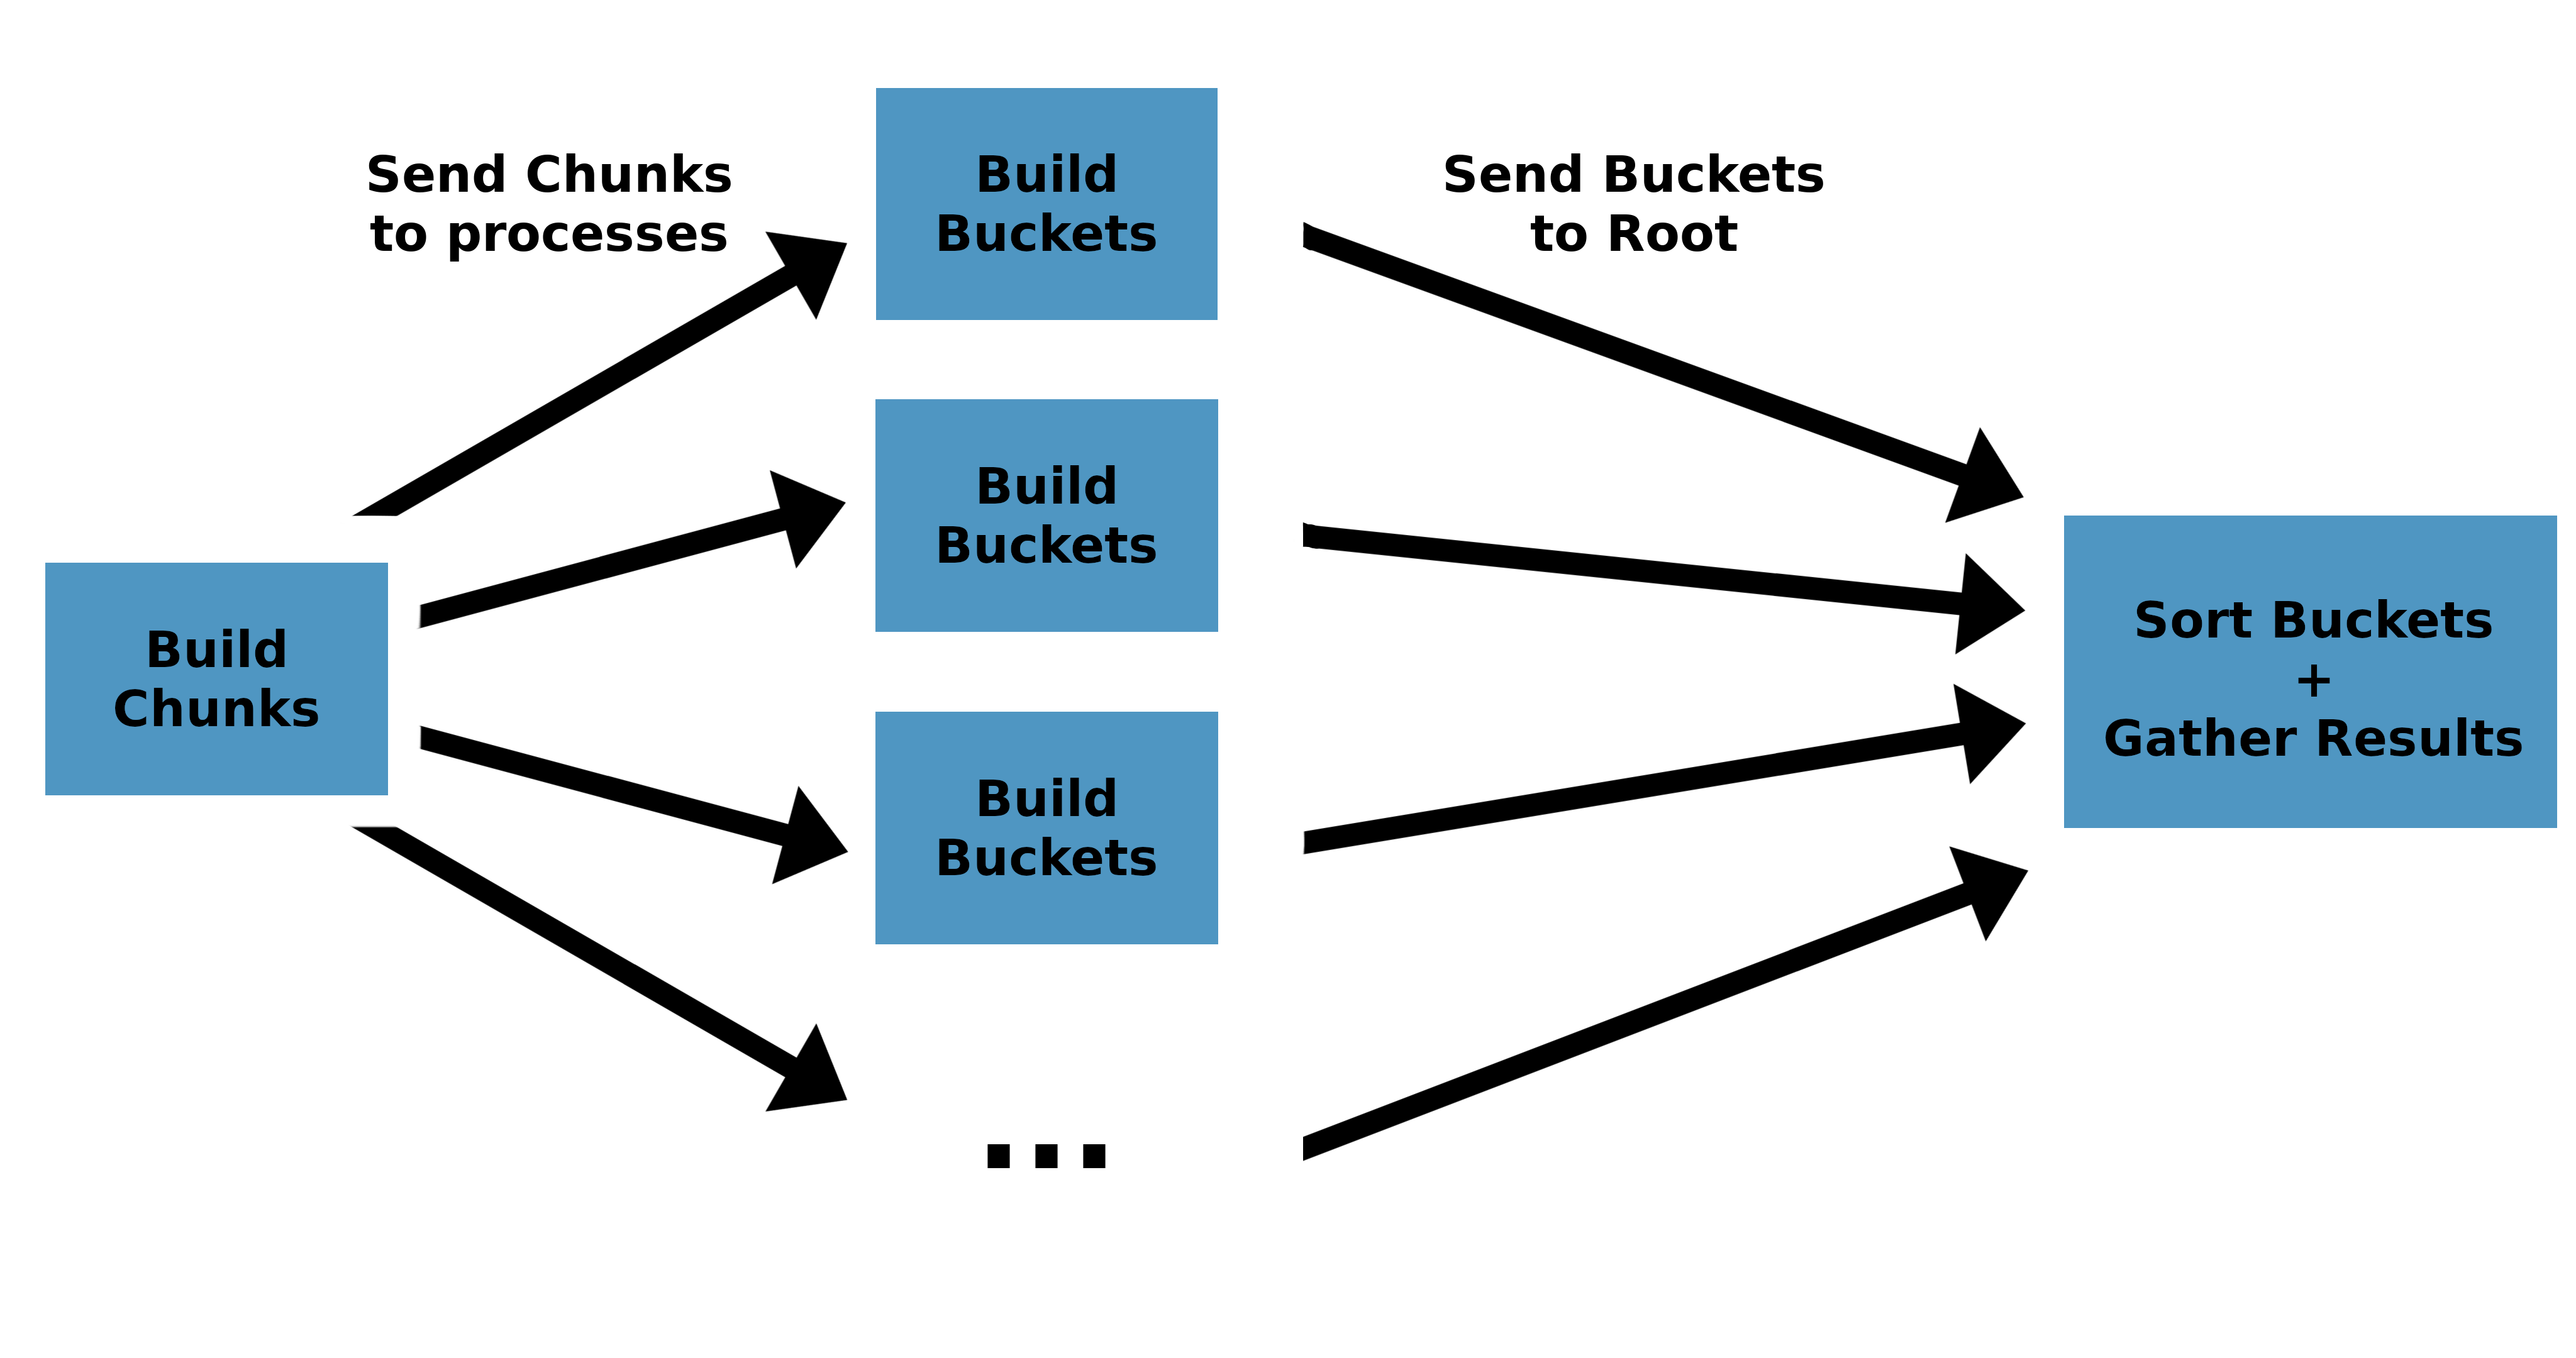
\includegraphics[width=0.5\textwidth]{images/esquemas/algoritmo_graph1.png}
    \caption{Arquitetura da Solução}
\end{figure}

\begin{table}[h]
    \centering
    \begin{tabular}{|c|c|}
        \hline
        Processes & Time(Seconds) \\ \hline
        2         & 14,002223     \\ \hline
        4         & 13,410518     \\ \hline
        8         & 13,971147     \\ \hline
        16        & 14,244233     \\ \hline
        32        & 14,635107     \\ \hline
    \end{tabular}
    \caption{Tempos de execução da versão inicial do algoritmo}
    \label{tab:oldtimes}
\end{table}

Como podemos ver na tabela \ref{tab:oldtimes}, os tempos de execução são todos
semelhantes, pelo que não houve nenhum speedup perante o aumento de processos.
Podemos concluir também que a parte com maior intensidade computacional do
algoritmo será a terceira fase, sendo a seguinte a ser paralelizada.

\end{document}
